\documentclass{beamer}
\usepackage[utf8]{inputenc}
\usepackage{graphicx, epsfig}
\usepackage{amsmath,mathrsfs,amsfonts,amssymb}
\usepackage{floatflt}
\usepackage{epic,ecltree}
\usepackage{mathtext}
\usepackage{fancybox}
\usepackage{fancyhdr}
\usepackage{multirow}
\usepackage{enumerate}
\usepackage{epstopdf}
\usepackage{multicol}
\usepackage{algorithm}
\usepackage[noend]{algorithmic}
\usepackage{tikz}
\usepackage{blindtext}
\usetheme{default}%{Singapore}%{Warsaw}%{Warsaw}%{Darmstadt}
\usecolortheme{default}

\setbeamerfont{title}{size=\Huge}
\setbeamertemplate{footline}[page number]{}

\setbeamertemplate{section in toc}[sections numbered]


\makeatletter
\newcommand\HUGE{\@setfontsize\Huge{35}{40}}
\makeatother    

\setbeamerfont{title}{size=\HUGE}
\beamertemplatenavigationsymbolsempty

% latin bold lower
\newcommand{\ba}{\mathbf{a}} 
\newcommand{\bc}{\mathbf{c}} 
\newcommand{\be}{\mathbf{e}} 
\newcommand{\bh}{\mathbf{h}} 
\newcommand{\bp}{\mathbf{p}} 
\newcommand{\bt}{\mathbf{t}} 
\newcommand{\bs}{\mathbf{s}} 
\newcommand{\bu}{\mathbf{u}} 
\newcommand{\bv}{\mathbf{v}} 
\newcommand{\bw}{\mathbf{w}} 
\newcommand{\bx}{\mathbf{x}} 
\newcommand{\by}{\mathbf{y}} 
\newcommand{\bz}{\mathbf{z}} 

% latin bold upper
\newcommand{\bA}{\mathbf{A}} 
\newcommand{\bB}{\mathbf{B}} 
\newcommand{\bC}{\mathbf{C}} 
\newcommand{\bI}{\mathbf{I}} 
\newcommand{\bL}{\mathbf{L}} 
\newcommand{\bM}{\mathbf{M}} 
\newcommand{\bQ}{\mathbf{Q}} 
\newcommand{\bT}{\mathbf{T}} 
\newcommand{\bU}{\mathbf{U}} 
\newcommand{\bV}{\mathbf{V}} 
\newcommand{\bW}{\mathbf{W}} 
\newcommand{\bX}{\mathbf{X}} 
\newcommand{\bY}{\mathbf{Y}} 
\newcommand{\bZ}{\mathbf{Z}} 

% latin cal upper
\newcommand{\cG}{\mathcal{G}} 
\newcommand{\cL}{\mathcal{L}} 
\newcommand{\cN}{\mathcal{N}} 
\newcommand{\cS}{\mathcal{S}} 
\newcommand{\cT}{\mathcal{T}} 
\newcommand{\cW}{\mathcal{W}} 
\newcommand{\cX}{\mathcal{X}} 
\newcommand{\cZ}{\mathcal{Z}} 

% latin bb upper
\newcommand{\bbE}{\mathbb{E}} 
\newcommand{\bbI}{\mathbb{I}} 
\newcommand{\bbP}{\mathbb{P}} 
\newcommand{\bbR}{\mathbb{R}} 

% greek bold lower
\newcommand{\bepsilon}{\boldsymbol{\epsilon}} 
\newcommand{\btheta}{\boldsymbol{\theta}} 
\newcommand{\blambda}{\boldsymbol{\lambda}} 
\newcommand{\bpi}{\boldsymbol{\pi}} 
\newcommand{\bmu}{\boldsymbol{\mu}} 
\newcommand{\bsigma}{\boldsymbol{\sigma}} 
\newcommand{\bphi}{\boldsymbol{\phi}} 

% greek bold upper
\newcommand{\bSigma}{\boldsymbol{\Sigma}} 

\DeclareMathOperator*{\argmin}{arg\,min}
\DeclareMathOperator*{\argmax}{arg\,max}

\newcommand{\createdgmtitle}[1]{\title[\hbox to 56mm{Deep Generative Models  \hfill\insertframenumber\,/\,\inserttotalframenumber}]
	{Deep Generative Models \\ {\Huge Lecture #1}}
	\author{Roman Isachenko}
	\institute{
\includegraphics[width=0.5cm]{../utils/ozonmasterslogo} \large{Ozon Masters}}
	\date{Spring, 2022}
}

\newcommand\myfootnote[1]{%
  \tikz[remember picture,overlay]
  \draw (current page.south west) +(1in + \oddsidemargin,0.5em)
  node[anchor=south west,inner sep=0pt]{\parbox{\textwidth}{%
      \rlap{\rule{10em}{0.4pt}}\raggedright\scriptsize \textit{#1}}};}

\newcommand\myfootnotewithlink[2]{%
  \tikz[remember picture,overlay]
  \draw (current page.south west) +(1in + \oddsidemargin,0.5em)
  node[anchor=south west,inner sep=0pt]{\parbox{\textwidth}{%
      \rlap{\rule{10em}{0.4pt}}\raggedright\scriptsize\href{#1}{\textit{#2}}}};}
      
\AtBeginSection[]
{
	\begin{frame}{Outline}
		\tableofcontents[currentsection,subsectionstyle=hide]
	\end{frame}
}
\AtBeginSubsection[]{
	\begin{frame}{Outline}
		\tableofcontents[currentsection,currentsubsection]
	\end{frame}
}
\createdgmtitle{10}
%--------------------------------------------------------------------------------
\begin{document}
%--------------------------------------------------------------------------------
\begin{frame}[noframenumbering,plain]
%\thispagestyle{empty}
\titlepage
\end{frame}
%=======
\begin{frame}{Recap of previous lecture}
	\begin{itemize}
		\item \textbf{Generator:} generative model $\bx = G(\bz)$, which makes generated sample more realistic.
		\item \textbf{Discriminator:} a classifier $D(\bx) \in [0, 1]$, which distinguishes real samples from generated samples.
	\end{itemize}
	
	\begin{block}{GAN optimality theorem}
		The minimax game 
		\vspace{-0.2cm}
		\[
			\min_{G} \max_D V(G, D) = \min_{G} \max_D \left[ \bbE_{\pi(\bx)} \log D(\bx) + \bbE_{p(\bz)} \log (1 - D(G(\bz))) \right]
		\]
		 has the global optimum $\pi(\bx) = p(\bx | \btheta)$, in this case $D^*(\bx) = 0.5$.
	\end{block}
	\vspace{-0.5cm}
	\[
		\min_{G} V(G, D^*) = \min_{G} \left[ 2 JSD(\pi || p) - \log 4 \right] = -\log 4, \quad \pi(\bx) = p(\bx | \btheta).
	\]
	\vspace{-0.4cm} \\
	If the generator could be any function and the discriminator is optimal at every step, then the generator is guaranteed to converge to the data distribution.
	 \myfootnotewithlink{https://arxiv.org/abs/1406.2661}{Goodfellow I. J. et al. Generative Adversarial Networks, 2014}
\end{frame}
%=======
\begin{frame}{Recap of previous lecture}
	\begin{block}{ELBO objective}
		\vspace{-0.5cm}
		\[
			 \mathcal{L} (\bphi, \btheta)  = \mathbb{E}_{q(\bz | \bx, \bphi)} \left[\log p(\bx | \bz, \btheta) + \log p(\bz) - \log q(\bz| \bx, \bphi) \right] \rightarrow \max_{\bphi, \btheta}.
		\]	
		\vspace{-0.5cm}
	\end{block}
	What is the problem to make the variational posterior model an \textbf{implicit} model? \\
	 We have to estimate density ratio 
	\[
		r(\bx, \bz) = \frac{q_1(\bx, \bz)}{q_2(\bx, \bz)} = \frac{p(\bz) \pi(\bx)}{q(\bz| \bx, \bphi) \pi (\bx)}.
	\] 
	\begin{block}{Adversarial Variational Bayes}
		\vspace{-0.6cm}
		\[
			\max_D \left[ \bbE_{\pi(\bx)} \bbE_{q(\bz | \bx, \bphi)} \log D(\bx, \bz) + \bbE_{\pi(\bx)} \bbE_{p(\bz)} \log (1 - D(\bx, \bz)) \right]
		\]
	\end{block}
	\myfootnotewithlink{https://arxiv.org/abs/1701.04722}{Mescheder L., Nowozin S., Geiger A. Adversarial variational bayes: Unifying variational autoencoders and generative adversarial networks, 2017}
\end{frame}
%=======
\begin{frame}{Recap of previous lecture}
	\begin{block}{Standard GAN}
		\vspace{-0.6cm}
		\[
			\min_{G} \max_D V(G, D) = \min_{G} \max_D \left[ \bbE_{\pi(\bx)} \log D(\bx) + \bbE_{p(\bz)} \log (1 - D(G(\bz))) \right]
		\]
		\vspace{-0.7cm}
	\end{block}
	\begin{block}{Main problems}
		\begin{itemize}
			\item Vanishing gradients (non-saturating GAN does not suffer of it);
			\item Mode collapse (caused by behaviour of Jensen-Shannon divergence).
		\end{itemize}
	\end{block}
	\vspace{-0.1cm}
	\begin{block}{Informal theoretical results}
		Distribution of real images $\pi(\bx)$ and distribution of generated images $p(\bx | \btheta)$ are low-dimensional and have disjoint supports. In this case
		\vspace{-0.3cm}
		\[
			KL(\pi || p) = KL(p || \pi) = \infty, \quad JSD(\pi || p) = \log 2
		\]
		\end{block}
		\myfootnote{\href{https://arxiv.org/abs/1406.2661}{Goodfellow I. J. et al. Generative Adversarial Networks, 2014} \\
		\href{https://arxiv.org/abs/1701.04862}{Arjovsky M., Bottou L. Towards Principled Methods for Training Generative Adversarial Networks, 2017}}
\end{frame}
%=======
\begin{frame}{Recap of previous lecture}
		\begin{block}{Wasserstein distance}
			\vspace{-0.5cm}
			\[
				W(\pi, p) = \inf_{\gamma \in \Gamma(\pi, p)} \bbE_{(\bx, \by) \sim \gamma} \| \bx - \by \| =  \inf_{\gamma \in \Gamma(\pi, p)} \int \| \bx - \by \| \gamma (\bx, \by) d \bx d \by
			\]
			\vspace{-0.5cm}
			\begin{itemize}
				\item $\Gamma(\pi, p)$ -- the set of all joint distributions $\Gamma (\bx, \by)$ with marginals $\pi$ and $p$ ($\int \gamma(\bx, \by) d \bx = p(\by)$, $\int \gamma(\bx, \by) d \by = \pi(\bx)$)
				\item $\gamma(\bx, \by)$ -- transportation plan (the amount of "dirt" that should be transported from point $\bx$ to point $\by$).
				\item $\gamma(\bx, \by)$ -- the amount, $\|\bx - \by \|$-- the distance.
			\end{itemize}
		\end{block}
		\begin{block}{Theorem (Kantorovich-Rubinstein duality)}
			\vspace{-0.2cm}
			\[
				W(\pi || p) = \frac{1}{K} \max_{\| f \|_L \leq K} \left[ \bbE_{\pi(\bx)} f(\bx)  - \bbE_{p(\bx)} f(\bx)\right],
			\]
			where $\| f \|_L \leq K$ are $K-$Lipschitz continuous functions ($f: \cX \rightarrow \bbR$).
		\end{block}
		\myfootnotewithlink{https://arxiv.org/abs/1701.07875}{Arjovsky M., Chintala S., Bottou L. Wasserstein GAN, 2017}
\end{frame}
%=======
\begin{frame}{Outline}
	\tableofcontents
\end{frame}
\AtBeginSection[ ]
{
	\begin{frame}{Outline}
		\tableofcontents[currentsection]
	\end{frame}
}
%=======
\section{WGAN with Gradient Penalty}
%=======
\begin{frame}{Wasserstein GAN with Gradient Penalty}
	\begin{block}{Weight clipping analysis}
		\begin{itemize}
			\item The critic ignores higher moments of the data distribution.
			\item The gradients either grow or decay exponentially.
		\end{itemize}
	\end{block}
	\vspace{-0.2cm}
	\begin{figure}
		\centering
		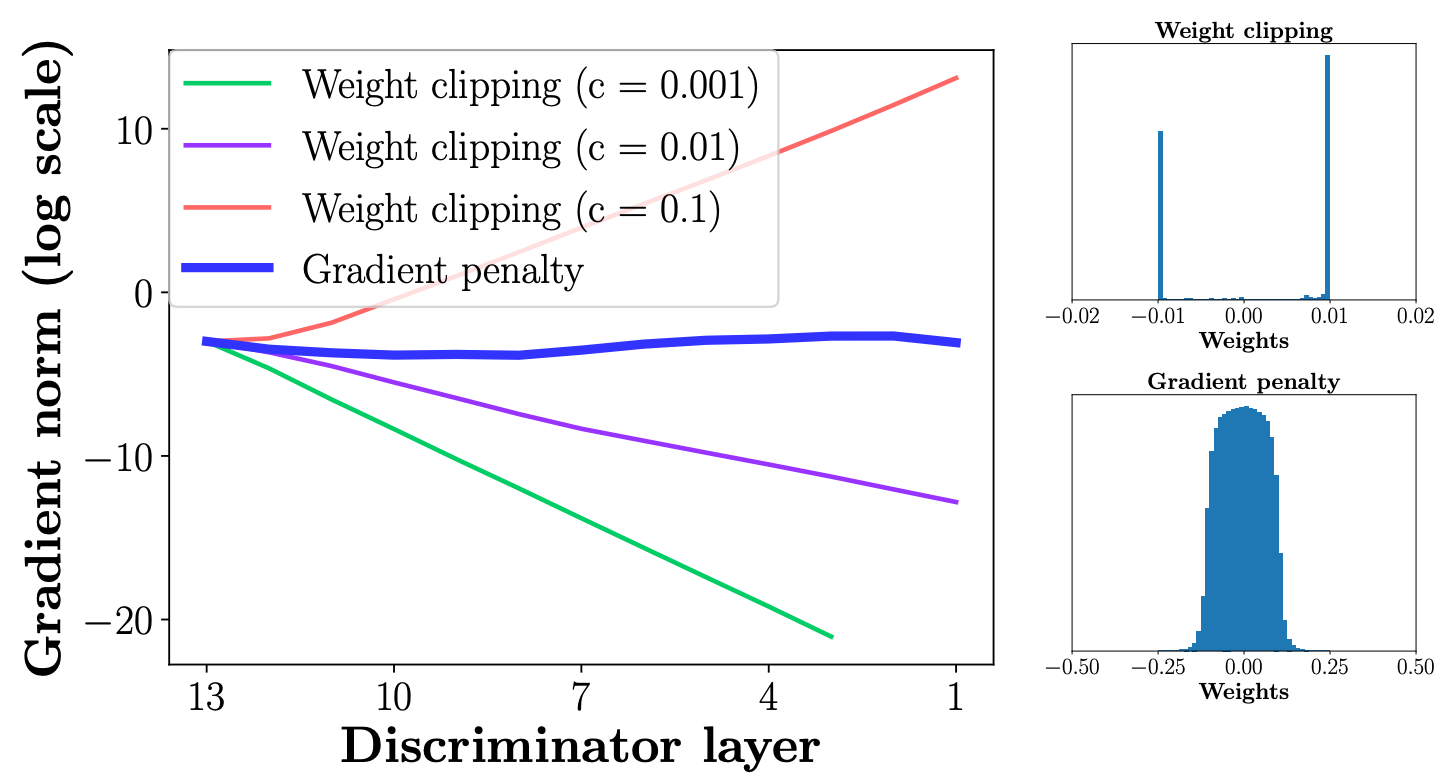
\includegraphics[width=0.8\linewidth]{figs/wgan_gp_weights}
	\end{figure}
	\vspace{-0.2cm} 
	
	Gradient penalty makes the gradients  more stable.
	\myfootnotewithlink{https://arxiv.org/abs/1704.00028}{Gulrajani I. et al. Improved Training of Wasserstein GANs, 2017}
\end{frame}
%=======
\begin{frame}{Wasserstein GAN with Gradient Penalty}
	\begin{block}{Theorem}
		Let $\pi(\bx)$ and $p(\bx)$ be two distribution in $\cX$, a compact metric space. Then, there is 1-Lipschitz function $f^*$ which is the optimal solution of 
		\[
			\max_{\| f \|_L \leq 1} \left[ \bbE_{\pi(\bx)} f(\bx)  - \bbE_{p(\bx)} f(\bx)\right].
		\]
		Let $\gamma$ be the optimal transportation plan between $\pi(\bx)$ and $p(\bx)$. Then, if $f^*$ is differentiable, $\gamma(\bx = \by) = 0$ and $\hat{\bx}_t = t \bx + (1 - t) \by$ with $\bx \sim \pi(\bx)$, $\by \sim p(\bx | \btheta)$, $t \in [0, 1]$ it holds that
		\[
			\bbP_{(\bx, \by) \sim \gamma} \left[ \nabla f^*(\hat{\bx}_t) = \frac{\by - \hat{\bx}_t}{\| \by - \hat{\bx}_t \|} \right] = 1.
		\]
	\end{block}
	\vspace{-0.2cm}
	\begin{block}{Corollary}
		$f^*$ has gradient norm 1 almost everywhere under $\pi(\bx)$ and $p(\bx)$.
	\end{block}

	\myfootnotewithlink{https://arxiv.org/abs/1704.00028}{Gulrajani I. et al. Improved Training of Wasserstein GANs, 2017}
\end{frame}
%=======
\begin{frame}{Wasserstein GAN with Gradient Penalty}
	A differentiable function is 1-Lipschtiz if and only if it has gradients with norm at most 1 everywhere.
	\begin{block}{Gradient penalty}
		\[
			W(\pi || p) = \underbrace{\bbE_{\pi(\bx)} f(\bx)  - \bbE_{p(\bx)} f(\bx)}_{\text{original critic loss}} + \lambda \underbrace{\bbE_{U[0, 1]} \left[ \left( \| \nabla_{\hat{\bx}} f(\hat{\bx}) \|_2 - 1 \right) ^ 2\right]}_{\text{gradient penalty}},
		\]
	\end{block}
	\begin{itemize}
		\item Samples $\hat{\bx}_t = t \bx + (1 - t) \by$ with $t \in [0, 1]$ are uniformly sampled along straight lines between pairs of points: $\bx$ from the data distribution $\pi(\bx)$ and $\by$ from the generator distribution $p(\bx | \btheta)$.
		\item Enforcing the unit gradient norm constraint everywhere is intractable, it turns out to be sifficient to enforce it only along these straight lines.
	\end{itemize}

	\myfootnotewithlink{https://arxiv.org/abs/1704.00028}{Gulrajani I. et al. Improved Training of Wasserstein GANs, 2017}
\end{frame}
%=======
\begin{frame}{Wasserstein GAN with Gradient Penalty}
	\begin{figure}
		\centering
		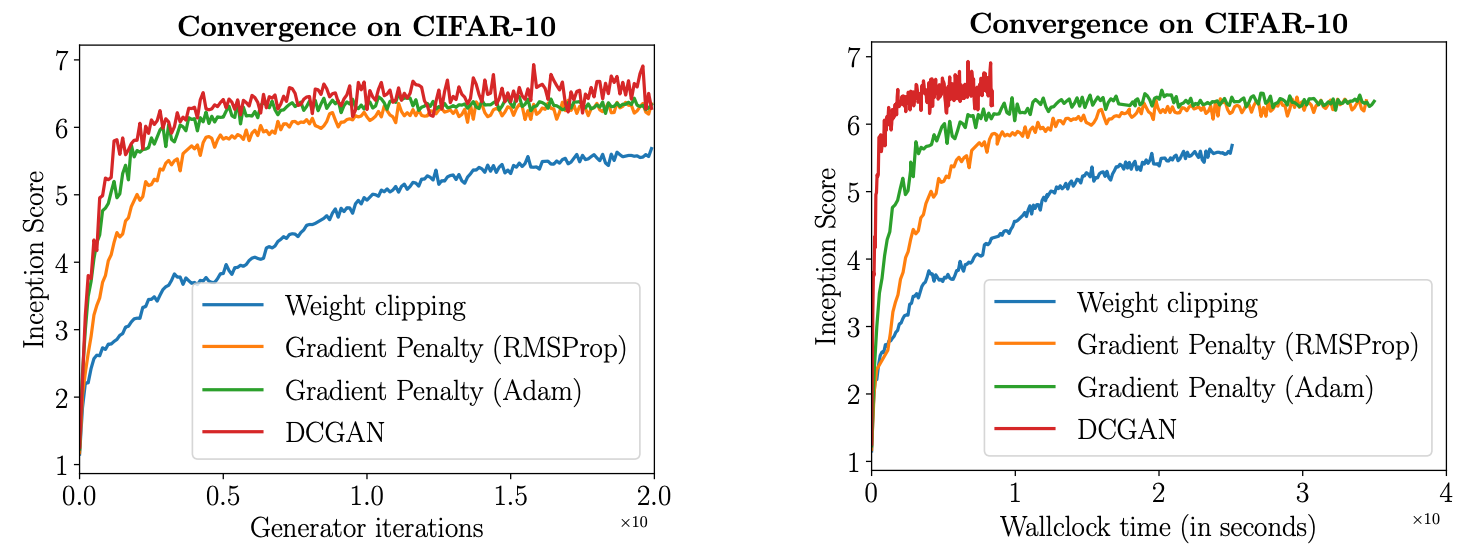
\includegraphics[width=\linewidth]{figs/wgan_gp_convergence}
	\end{figure}
	\begin{block}{WGAN-GP convergence}
		\begin{figure}
			\centering
			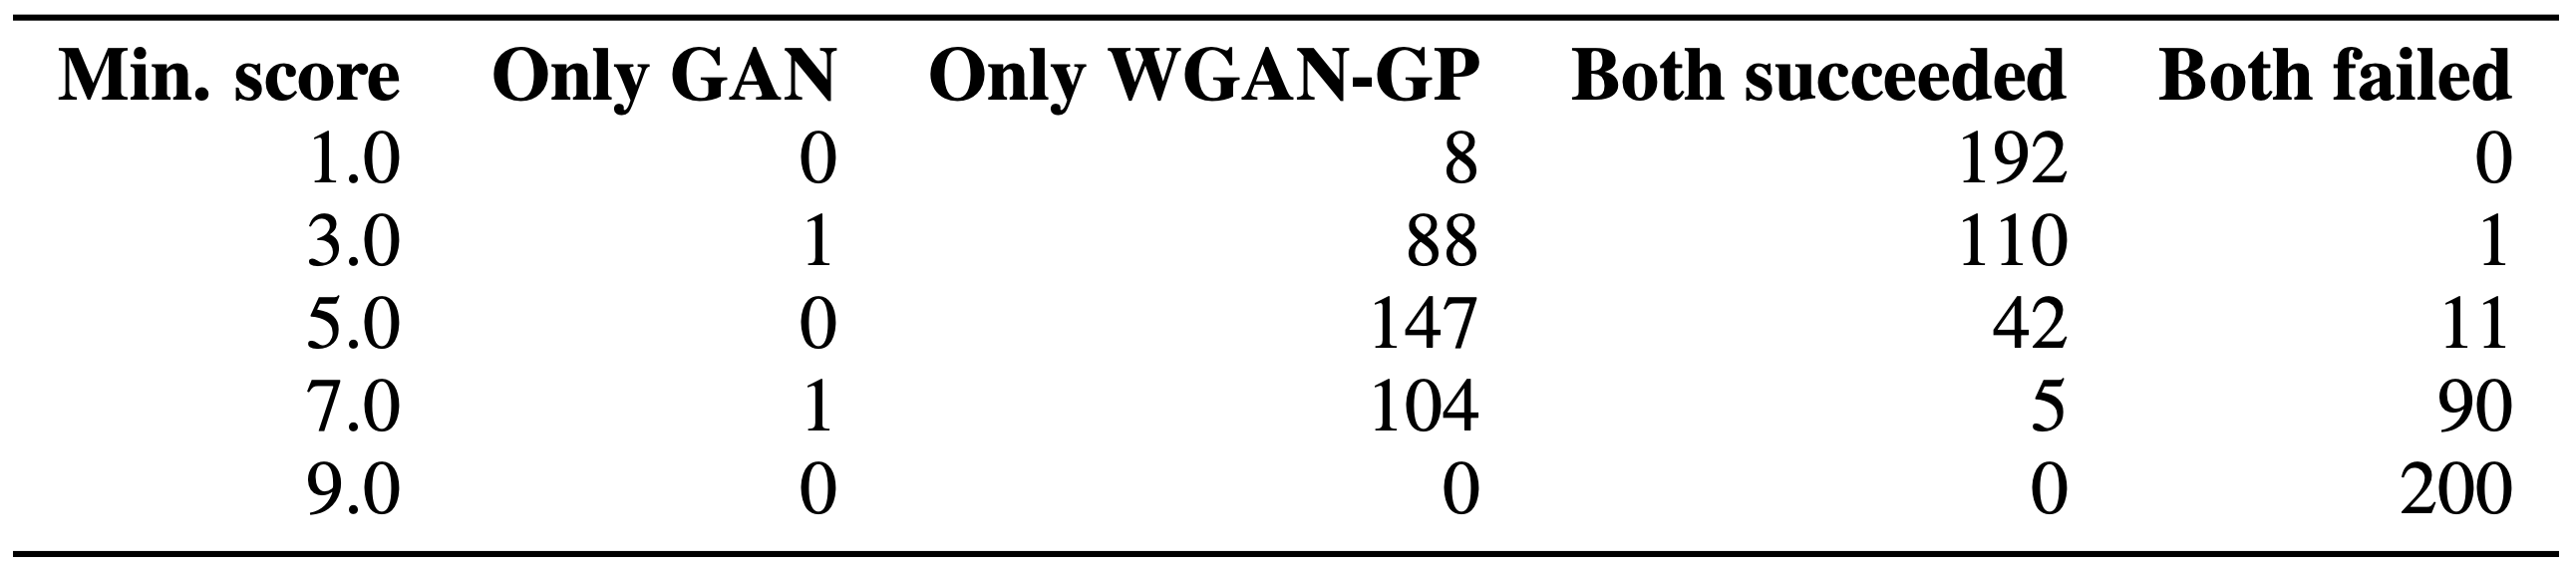
\includegraphics[width=0.75\linewidth]{figs/wgan_gp_wgan}
		\end{figure}
	\end{block}

	\myfootnotewithlink{https://arxiv.org/abs/1704.00028}{Gulrajani I. et al. Improved Training of Wasserstein GANs, 2017}
\end{frame}
%=======
\begin{frame}{Spectral Normalization GAN}
	\begin{block}{Definition}
		$\| \bA \|_2$ is a \textit{spectral norm} of matrix $\bA$:
		\[
			\| \bA \|_2 = \max_{\bh \neq 0} \frac{\|\bA \bh\|_2}{\|\bh\|_2} = \max_{\|\bh\|_2 \leq 1} \| \bA \bh \|_2 = \lambda_{\text{max}}(\bA^T \bA),
		\]
		where $\lambda_{\text{max}}(\bA^T \bA)$ is the largest eigenvalue value of $\bA^T \bA$.
	\end{block}
	\begin{block}{Statement 1}
		if $g$ is a K-Lipschitz function then 
		\[
			\| \mathbf{g} \|_L \leq K = \sup_\bx \| \nabla \mathbf{g}(\bx)) \|_2.
		\]
		\vspace{-0.7cm}
	\end{block}
	\begin{block}{Statement 2}
		Lipschitz norm of superposition is bounded above by product of Lipschitz norms
		\vspace{-0.2cm}
		\[
			\| \mathbf{g}_1 \circ \mathbf{g}_2 \|_L \leq \| \mathbf{g}_1 \|_L \cdot \| \mathbf{g}_2\|_L
		\]
	\end{block}
	\myfootnotewithlink{https://arxiv.org/abs/1802.05957}{Miyato T. et al. Spectral Normalization for Generative Adversarial Networks, 2018}
\end{frame}
%=======
\section{Spectral Normalization GAN}
%=======
\begin{frame}{Spectral Normalization GAN}
	Let consider the critic $f(\bx, \bphi)$ of the following form:
	\[
		f(\bx, \bphi) = \bW_{K+1} \sigma_K (\bW_K \sigma_{K-1}(\dots \sigma_1(\bW_1 \bx) \dots)).
	\]
	This feedforward network is a superposition of simple functions.
	\begin{itemize}
		\item $\sigma_k$ is a pointwise nonlinearities. We assume that $\| \sigma_k \|_L = 1$ (it holds for ReLU).
		\item $\mathbf{g}(\bx) = \bW \bx$ is a linear transformation ($\nabla \mathbf{g}(\bx) = \bW$).
		\[
			\| \mathbf{g} \|_L \leq \sup_\bx \| \nabla \mathbf{g}(\bx)\|_2 = \| \bW \|_2.
		\]
	\end{itemize}
	\vspace{-0.4cm}
	\begin{block}{Critic spectral norm}
		\vspace{-0.4cm}
		\[
			\| f \|_L \leq \| \bW_{K+1}\| \cdot \prod_{k=1}^K  \| \sigma_k \|_L \cdot \| \bW_k \|_2 = \prod_{k=1}^{K+1} \|\bW_k\|_2.
		\]
		\vspace{-0.2cm}
	\end{block}
	If we replace the weights in the critic $f(\bx, \bphi)$ by $\bW^{SN}_k = \bW_k / \|\bW_k\|_2$, we will get $\| f\|_L \leq 1.$ \\
	
	\myfootnotewithlink{https://arxiv.org/abs/1802.05957}{Miyato T. et al. Spectral Normalization for Generative Adversarial Networks, 2018}
\end{frame}
%=======
\begin{frame}{Spectral Normalization GAN}
	How to compute $ \| \bW \|_2 = \lambda_{\text{max}}(\bW^T \bW)$? \\
	 If we apply SVD to compute the $\| \bW \|_2$ at each iteration, the algorithm becomes intractable.
	 
	 \begin{block}{Power iteration method}
	 	\begin{itemize}
	 		\item $\bu_0$ -- random vector.
	 		\item for $k = 0, \dots, n - 1$: ($n$ is a large enough number of steps)
	 		\[
	 			\bv_{k+1} = \frac{\bW^T \bu_{k}}{\| \bW^T \bu_{k} \|}, \quad \bu_{k+1} = \frac{\bW \bv_{k+1}}{\| \bW \bv_{k+1} \|}.
	 		\]
	 		\item approximate the spectral norm
	 		\[
	 			\| \bW \|_2 = \lambda_{\text{max}}(\bW^T \bW) \approx \bu_{n}^T \bW \bv_{n}.
	 		\]
	 	\end{itemize}
	 \end{block}

	\myfootnotewithlink{https://arxiv.org/abs/1802.05957}{Miyato T. et al. Spectral Normalization for Generative Adversarial Networks, 2018}
\end{frame}
%=======
\begin{frame}{Spectral Normalization GAN}
	\begin{figure}
		\centering
		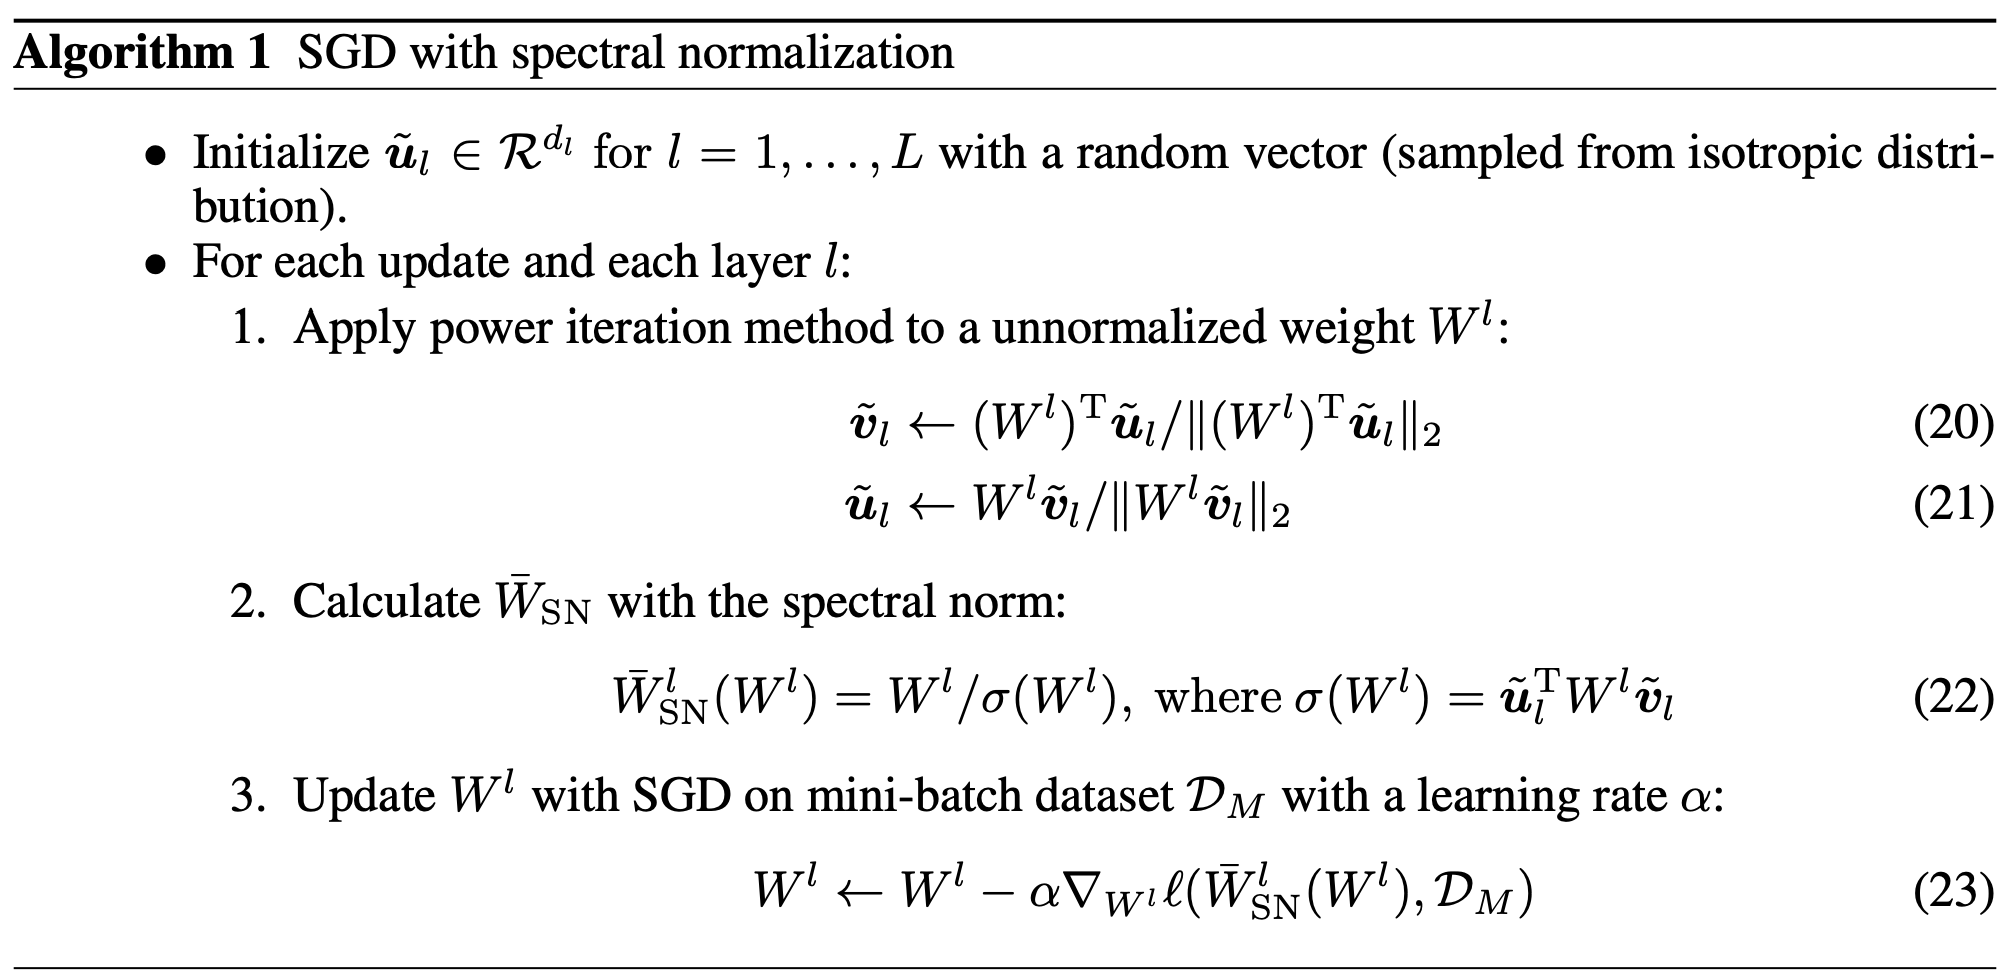
\includegraphics[width=0.85\linewidth]{figs/sngan_pseudocode}
	\end{figure}
	\begin{figure}
		\centering
		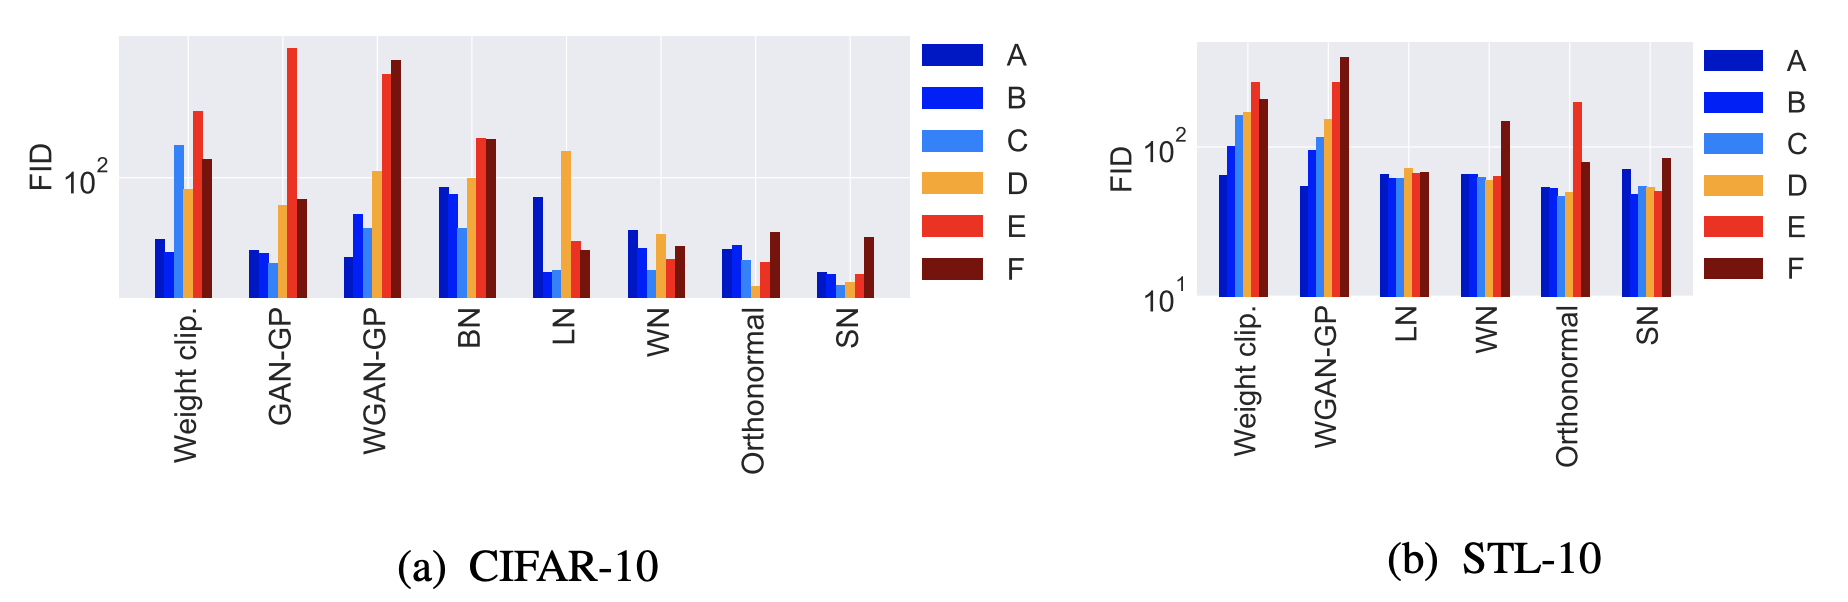
\includegraphics[width=0.85\linewidth]{figs/sngan_fids}
	\end{figure}

	\myfootnotewithlink{https://arxiv.org/abs/1802.05957}{Miyato T. et al. Spectral Normalization for Generative Adversarial Networks, 2018}
\end{frame}
%=======
\section{f-divergence minimization}
%=======
\begin{frame}{Divergences}
	\begin{itemize}
		\item Forward KL divergence in maximum likelihood estimation.
		\item Reverse KL in variational inference.
		\item JS divergence in standard GAN.
		\item Wasserstein distance in WGAN.
	\end{itemize}
	\begin{block}{What is a divergence?}
		Let $\cS$ be the set of all possible probability distributions. Then $D: \cS \times \cS \rightarrow \bbR$ is a divergence if 
		\begin{itemize}
			\item $D(\pi || p) \geq 0$ for all $\pi, p \in \cS$;
			\item $D(\pi || p) = 0$ if and only if $\pi \equiv p$.
		\end{itemize}
	\end{block}
	\begin{block}{General divergence minimization task}
		\vspace{-0.3cm}
		\[
			\min_p D(\pi || p)
		\]
		\vspace{-0.7cm}
	\end{block}
	\begin{block}{Chalenge}
		We do not know the real distribution $\pi(\bx)$!
	\end{block}
\end{frame}
%=======
\begin{frame}{f-divergence family}
	
	\begin{block}{f-divergence}
		\vspace{-0.3cm}
		\[
		D_f(\pi || p) = \bbE_{p(\bx)}  f\left( \frac{\pi(\bx)}{p(\bx)} \right)  = \int p(\bx) f\left( \frac{\pi(\bx)}{p(\bx)} \right) d \bx.
		\]
		Here $f: \bbR_+ \rightarrow \bbR$ is a convex, lower semicontinuous function satisfying $f(1) = 0$.
	\end{block}
	\begin{figure}
		\centering
		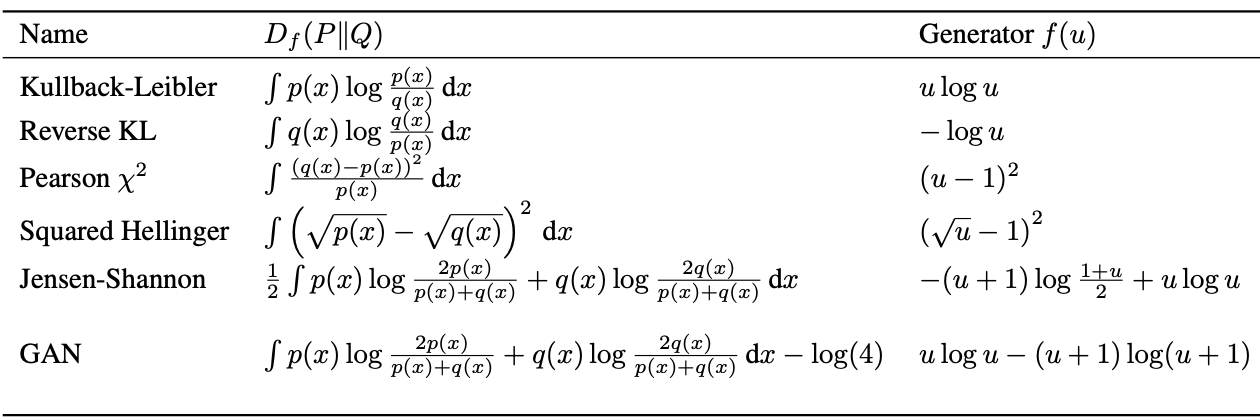
\includegraphics[width=\linewidth]{figs/f_divs}
	\end{figure}
	\myfootnotewithlink{https://arxiv.org/abs/1606.00709}{Nowozin S., Cseke B., Tomioka R. f-GAN: Training Generative Neural Samplers using Variational Divergence Minimization, 2016}
\end{frame}
%=======
\begin{frame}{f-divergence family}
	\vspace{-0.2cm}
	\begin{block}{Fenchel conjugate}
		\vspace{-0.7cm}
		\[
		f^*(t) = \sup_{u \in \text{dom}_f} \left( ut - f(u) \right), \quad f(u) = \sup_{t \in \text{dom}_{f^*}} \left( ut - f^*(t) \right)
		\]
		\vspace{-0.5cm}
	\end{block}
	\textbf{Important property:} $ f^{**} = f$ for convex $f$.
	\begin{block}{f-divergence}
		\vspace{-0.8cm}
		\begin{multline*}
			D_f(\pi || p) = \bbE_{p(\bx)}  f\left( \frac{\pi(\bx)}{p(\bx)} \right)  = \int p(\bx) f\left( \frac{\pi(\bx)}{p(\bx)} \right) d \bx = \\ = \int p(\bx) \sup_{t \in \text{dom}_{f^*}} \left( \frac{\pi(\bx)}{p(\bx)} t - f^*(t) \right) d \bx = \\ 
			= \int \sup_{t \in \text{dom}_{f^*}} \left( \pi(\bx)t - p(\bx) f^*(t) \right) d \bx .
		\end{multline*}
		\vspace{-0.6cm}
	\end{block}
	Here we seek value of $t$, which gives us maximum value of $ \pi(\bx)t - p(\bx) f^*(t)$, for each data point $\bx$.
	\myfootnotewithlink{https://arxiv.org/abs/1606.00709}{Nowozin S., Cseke B., Tomioka R. f-GAN: Training Generative Neural Samplers using Variational Divergence Minimization, 2016}
\end{frame}
%=======
\begin{frame}{f-divergence family}
	\vspace{-0.4cm}
	\begin{block}{f-divergence}
		\vspace{-0.3cm}
		\[
		D_f(\pi || p) = \bbE_{p(\bx)}  f\left( \frac{\pi(\bx)}{p(\bx)} \right)  = \int p(\bx) f\left( \frac{\pi(\bx)}{p(\bx)} \right) d \bx.
		\]
		\vspace{-0.4cm}
	\end{block}
	\begin{block}{Variational f-divergence estimation}
		\vspace{-0.8cm}
		\begin{multline*}
			D_f(\pi || p)  = \int \sup_{t \in \text{dom}_{f^*}} \left( \pi(\bx)t - p(\bx) f^*(t) \right) d \bx \geq \\
			 \geq \sup_{T \in \cT} \int \left( \pi(\bx)T(\bx) - p(\bx) f^*(T(\bx)) \right) d \bx = \\
			 = \sup_{T \in \cT} \left[\bbE_{\pi}T(\bx) -  \bbE_p f^*(T(\bx)) \right]
		\end{multline*}
	\vspace{-0.6cm}
	\end{block}
	This is a lower bound because of Jensen-Shannon inequality and restricted class of functions $\cT: \cX \rightarrow \bbR$.
	
	\myfootnotewithlink{https://arxiv.org/abs/1606.00709}{Nowozin S., Cseke B., Tomioka R. f-GAN: Training Generative Neural Samplers using Variational Divergence Minimization, 2016}
\end{frame}
%=======
\begin{frame}{f-divergence family}
	\begin{block}{Variational divergence estimation}
		\[
			D_f(\pi || p) \geq \sup_{T \in \cT} \left[\bbE_{\pi}T(\bx) -  \bbE_p f^*(T(\bx)) \right]
		\]
		The lower bound is tight for $T^*(\bx) = f'\left( \frac{\pi(\bx)}{p(\bx)} \right)$.
	\end{block}
	\begin{block}{Example (JSD)}
		\begin{itemize}
			\item Let define function $f$ and its conjugate $f^*$
			\[ 
				f(u) = u \log u - (u + 1) \log (u + 1), \quad f^*(t) = - \log (1 - e^t).
			\]
			\item Let reparametrize $T(\bx) = \log D(\bx)$.
		\end{itemize}
		\vspace{-0.7cm}
	\end{block}
	\[
		\min_{G} \max_D V(G, D) = \min_{G} \max_D \left[ \bbE_{\pi(\bx)} \log D(\bx) + \bbE_{p(\bz)} \log (1 - D(G(\bz))) \right]
	\]

	\myfootnotewithlink{https://arxiv.org/abs/1606.00709}{Nowozin S., Cseke B., Tomioka R. f-GAN: Training Generative Neural Samplers using Variational Divergence Minimization, 2016}
\end{frame}
%=======
\begin{frame}{f-divergence family}
	\begin{block}{Variational divergence estimation}
		\[
			D_f(\pi || p) \geq \sup_{T \in \cT} \left[\bbE_{\pi}T(\bx) -  \bbE_p f^*(T(\bx)) \right]
		\]
	\end{block}
	\textbf{Note:} To evaluate lower bound we only need samples from $\pi(\bx)$ and $p(\bx)$. Hence, we could fit implicit generative model.
	\begin{figure}
		\centering
		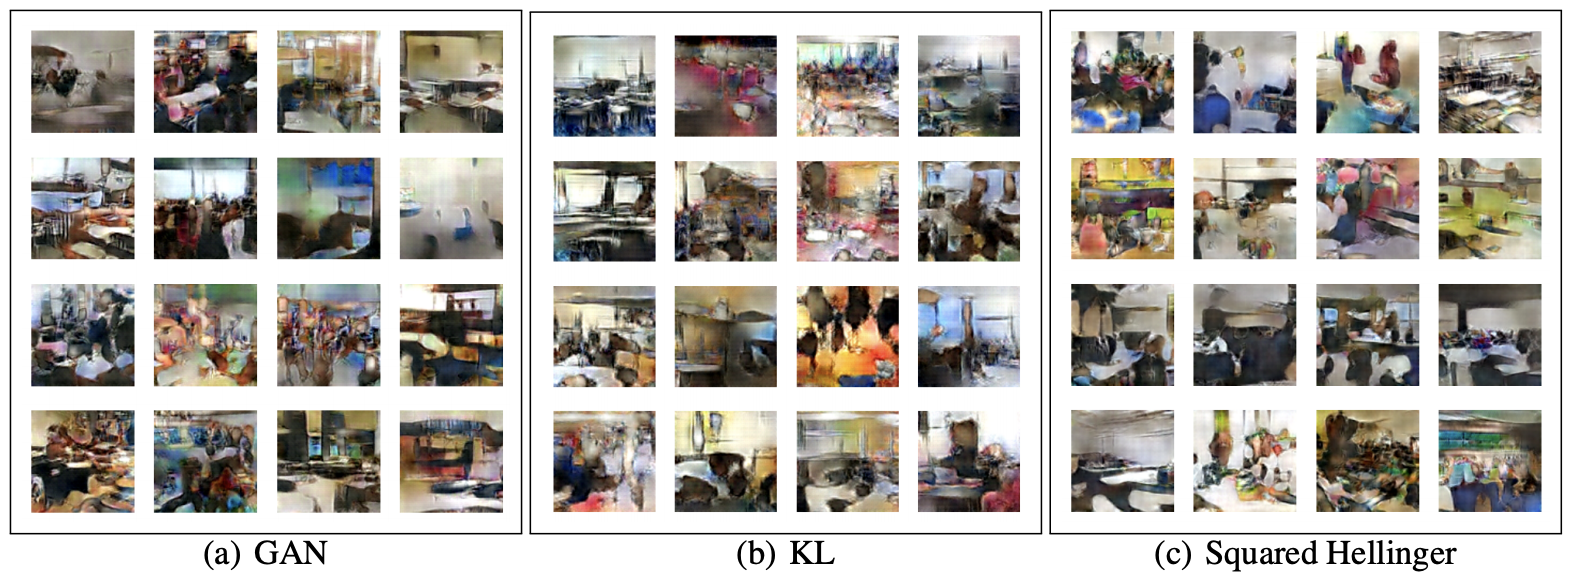
\includegraphics[width=1.0\linewidth]{figs/f_div_results}
	\end{figure}

	\myfootnotewithlink{https://arxiv.org/abs/1606.00709}{Nowozin S., Cseke B., Tomioka R. f-GAN: Training Generative Neural Samplers using Variational Divergence Minimization, 2016}
\end{frame}
%=======
\begin{frame}{Summary}
	\begin{itemize} 
		\item Weight clipping is a terrible way to enforce Lipschitzness. Gradient Penalty works better.
		\vfill
		\item Spectral normalization is a weight normalization technique to enforce Lipshitzness, which is helpful for generator and discriminator.
		\vfill
		\item f-divergence family is a unified framework for divergence minimization, which uses variational approximation. Standard GAN is a special case of it.
	\end{itemize}
\end{frame}
%=======
\end{document} 